Cada autovector que buscamos, proporciona nueva informaci\'on para nuestro an\'alisis. En esta secci\'on vamos a intentar ver cu\'al es esta informaci\'on, es decir, qu\'e es lo que nos est\'a diciendo cada autovector.

Vamos a tomar \'unicamente los primeros 3 autovectores obtenidos por cada m\'etodo, porque no se pueden graficar puntos en m\'as de 3 dimensiones.

\begin{table}[h!]
\begin{center}
\begin{tabular}{|c|c|c|}
	\hline
	\# & PCA & PLS-DA \\
	\hline
	Primer Autod\'igito &
	
\includegraphics[scale=4.00]{exp3/PCA-1} &
	
\includegraphics[scale=4.00]{exp3/PLS-1} \\
	\hline
	Segundo Autod\'igito &
	
\includegraphics[scale=4.00]{exp3/PCA-2} &
	
\includegraphics[scale=4.00]{exp3/PLS-2} \\
	\hline
	Tercer Autod\'igito &
	
\includegraphics[scale=4.00]{exp3/PCA-3} &
	
\includegraphics[scale=4.00]{exp3/PLS-3} \\
	\hline
\end{tabular}
\end{center}
\caption{Primeros autod\'igitos de los m\'etodos}
\end{table}

La tabla anterior muestra los 3 primeros autod\'igitos obtenidos para cada m\'etodo. Para obtener cada uno, se obtuvo el autovector asociado a cada uno de los primeros 3 autovalores, que est\'an normalizados. Se los convierte a base 0 - 1 \footnote{$(x^{i} - x_{min}) / (x_{max} - x_{min})$, con $x_{min}$ el m\'inimo valor encontrado en x y $x_{max}$ el m\'aximo, $x^{i}$ el $i$-\'esimo elemento de x} y se los multiplica por 255. As\'i obtenemos una matriz con valores entre 0 y 255 que representa una imagen, en particular la de los autod\'igitos.

\textbf{Hip\'otesis:} Dada la forma del primer autod\'igito, el primer autovector no admite confusi\'on entre los d\'igitos 0 y 1.

Para ver si esto vale, vamos a mostrar el extracto pertinente de las matrices de confusi\'on obtenidas para PCA y PLS-DA respectivamente:

\begin{table}[h!]
\begin{subtable}{.5\linewidth}
\begin{tabular}{|c|c|c|}
	\hline
	Actual\textbackslash Predicted & 0 & 1 \\
	\hline
	0 & 3009 & 0 \\
	\hline
	1 & 0 & 4091 \\
	\hline
\end{tabular}
\end{subtable}
\begin{subtable}{.5\linewidth}
\begin{tabular}{|c|c|c|}
	\hline
	Actual\textbackslash Predicted & 0 & 1 \\
	\hline
	0 & 3213 & 0 \\
	\hline
	1 & 0 & 3924 \\
	\hline
\end{tabular}
\end{subtable}
\end{table}

Se puede apreciar que la confusi\'on entre ambos d\'igitos es nula, el resto de la matriz no aporta grandes resultados, a excepci\'on que para el d\'igito 1:

Para PCA:

\begin{table}[h!]
\begin{tabular}{|c|c|c|c|c|c|c|c|c|c|c|}
	\hline
	Actual\textbackslash Predicted & 0 & 1 & 2 & 3 & 4 & 5 & 6 & 7 & 8 & 9 \\
	\hline
	1 & 0 & 3649 & 57 & 44 & 151 & 45 & 61 & 374 & 65 & 238 \\
	\hline
\end{tabular}
\end{table}

Para PLS-DA

\begin{table}[h!]
\begin{tabular}{|c|c|c|c|c|c|c|c|c|c|c|}
	\hline
	Actual\textbackslash Predicted & 0 & 1 & 2 & 3 & 4 & 5 & 6 & 7 & 8 & 9 \\
	\hline
	1 & 0 & 3924 & 8 & 25 & 91 & 7 & 7 & 421 & 24 & 177 \\
	\hline
\end{tabular}
\end{table}

Muestran que cuando la imagen a etiquetar es un 1, en la mayor\'ia de los casos va a acertar, pero si no lo hace, es m\'as probable que lo confunda con un 7 o con un 9, lo cual tiene sentido ya que los d\'igitos se parecen en su forma.

Es interesante entonces mostrar como se distribuyen los puntos en el nuevo espacio \footnote{El eje $y$ no es representativo, se tomo para simular $\mathbb{R}^{2}$}.

\begin{figure}[h!]
  \begin{center}
	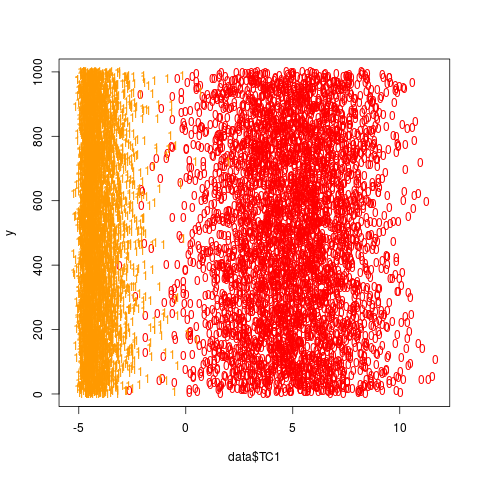
\includegraphics[scale=0.8]{exp5/PCA-1-0vs1}
	\caption{0 VS 1. Puntos en el nuevo espacio PCA}
  \end{center}
\end{figure}

\newpage

\begin{figure}[h!]
  \begin{center}
	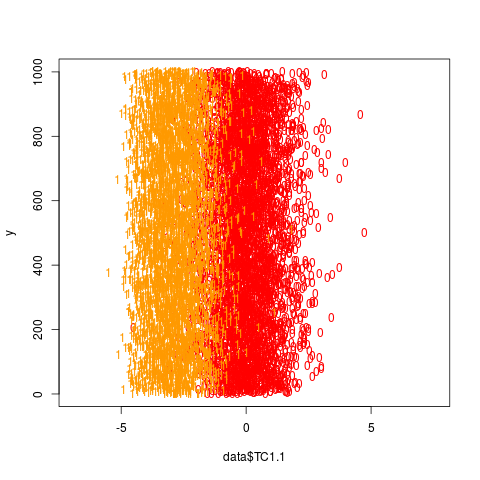
\includegraphics[scale=0.8]{exp5/PLS-1-0vs1}
	\caption{0 VS 1. Puntos en el nuevo espacio PLS-DA}
  \end{center}
\end{figure}

En PCA se ve una clara distancia entre los puntos transformados con etiquetas 0 y 1, guiados por el rasgo distintivo del autod\'igito. En PLS-DA parecer\'ia que se confunden en la frontera, aunque la mayor densidad de puntos est\'a en la media de cada uno, por lo que kNN clasificando un punto sobre la frontera no deber\'ia tener problemas \footnote{No pudimos encontrar una explicaci\'on para este fen\'omeno, creemos que la mayor\'ia de los 1's que se acercan a la media del 0 est\'an en la base de entrenamiento}.\\

Si el problema fuera clasificar 0's de 1's, con el primer autovector deber\'ia alcanzar, pero como pretendemos extender esto clasificar todos los d\'igitos, buscamos el segundo, que para ambos casos tiene forma de 9.

Como antes, mostramos las matrices de confusi\'on.

\newpage

\begin{table}[h!]
\begin{tabular}{|c|c|c|c|c|c|c|c|c|c|c|}
    \hline
    Actual\textbackslash Predicted & 0 & 1 & 2 & 3 & 4 & 5 & 6 & 7 & 8 & 9 \\
    \hline
    0 & 3080 & 1 & 282 & 71 & 7 & 175 & 414 & 4 & 92 & 6 \\
    \hline
    1 & 0 & 4353 & 66 & 46 & 15 & 54 & 19 & 33 & 85 & 13 \\
    \hline
    2 & 448 & 102 & 1017 & 792 & 92 & 538 & 494 & 48 & 609 & 37 \\
    \hline
    3 & 117 & 90 & 532 & 2098 & 60 & 437 & 293 & 39 & 660 & 25 \\
    \hline
    4 & 8 & 57 & 40 & 17 & 1704 & 91 & 216 & 820 & 43 & 1076 \\
    \hline
    5 & 359 & 78 & 527 & 609 & 181 & 701 & 633 & 62 & 560 & 85 \\
    \hline
    6 & 516 & 76 & 460 & 253 & 204 & 531 & 1299 & 58 & 661 & 79 \\
    \hline
    7 & 1 & 131 & 29 & 39 & 1109 & 98 & 103 & 1842 & 62 & 987 \\
    \hline
    8 & 273 & 109 & 553 & 703 & 121 & 568 & 653 & 41 & 984 & 58 \\
    \hline
    9 & 34 & 83 & 34 & 13 & 1383 & 92 & 154 & 1246 & 53 & 1096 \\
    \hline
\end{tabular}
\caption{Confusion Matrix PCA}
\end{table}

\begin{table}[h!]
\begin{tabular}{|c|c|c|c|c|c|c|c|c|c|c|}
    \hline
    Actual\textbackslash Predicted & 0 & 1 & 2 & 3 & 4 & 5 & 6 & 7 & 8 & 9 \\
    \hline
    0 & 3247 & 1 & 146 & 45 & 13 & 190 & 442 & 2 & 42 & 4 \\
    \hline
    1 & 0 & 4429 & 63 & 46 & 8 & 23 & 13 & 17 & 79 & 6 \\
    \hline
    2 & 247 & 127 & 1167 & 802 & 82 & 529 & 540 & 48 & 594 & 41 \\
    \hline
    3 & 60 & 89 & 569 & 2005 & 51 & 422 & 346 & 53 & 714 & 42 \\
    \hline
    4 & 7 & 34 & 29 & 33 & 1754 & 100 & 140 & 781 & 70 & 1124 \\
    \hline
    5 & 285 & 45 & 508 & 546 & 180 & 732 & 828 & 47 & 581 & 43 \\
    \hline
    6 & 499 & 64 & 460 & 364 & 155 & 694 & 1167 & 34 & 665 & 35 \\
    \hline
    7 & 4 & 90 & 23 & 36 & 1030 & 63 & 60 & 1949 & 70 & 1076 \\
    \hline
    8 & 184 & 120 & 504 & 763 & 170 & 553 & 676 & 58 & 974 & 61 \\
    \hline
    9 & 26 & 32 & 29 & 31 & 1346 & 75 & 102 & 1288 & 53 & 1206 \\
    \hline
\end{tabular}
\caption{Confusion Matrix PLS-DA}
\end{table}

Como primera impresi\'on de ambas tablas notamos que no se confunde 0 con 1 ni 1 con 0 salvo en un caso que debe ser un punto aislado en la muestra.

Lo destacable aqu\'i es que los 4, 7 y 9 o bien acierta o bien los confunde entre s\'i, salvo un peque\~no porcentaje de la muestra (razonable pues a\'un no tenemos mucha informaci\'on). Estos tres n\'umeros tienen la particularidad de un ``palo" que los distingue de los otros, el 1 tambi\'en lo tiene, pero este suele escribirse como un ``palo" mientras que los otros tres son un ``palo'' m\'as ``alg\'un garabato'' extra.

De esto podemos decir que el segundo autod\'igito distingue entre 4, 7 y 9 de los dem\'as.

\newpage

\begin{figure}[h!]
  \begin{center}
	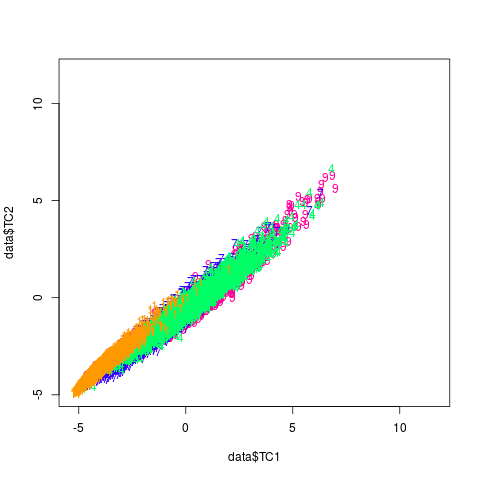
\includegraphics[scale=0.8]{exp5/PCA-2-1vs4vs7vs9}
	\caption{1 VS 4 VS 7 VS 9. Puntos en el nuevo espacio PCA}
  \end{center}
\end{figure}

Este es el espacio al que llegan los 4, 7 y 9 \footnote{el eje $y$ son los puntos que genera el segundo autovector}, casi que se superponen entre s\'i. Mientras el 1 est\'a superpuesto de alguna manera, pero en un sector m\'as chico, donde es m\'as denso y por ende, predominante.

En el siguiente gr\'afico, se ve que la superposici\'on para PLS-DA no se da tanto para el 1, lo cual se refleja en la matriz de confusi\'on que indica que hay menos confusiones de 4, 7 y/o 9 con el 1 que con PCA.

Esto adem\'as trae a la luz que ahora es m\'as dificil confundir al 1 con los dem\'as, pues con los que m\'as compet\'ia eran el 4, 7 y 9 y ahora estos fueron aislados a otro lugar del espacio.

\newpage

\begin{figure}[h!]
  \begin{center}
	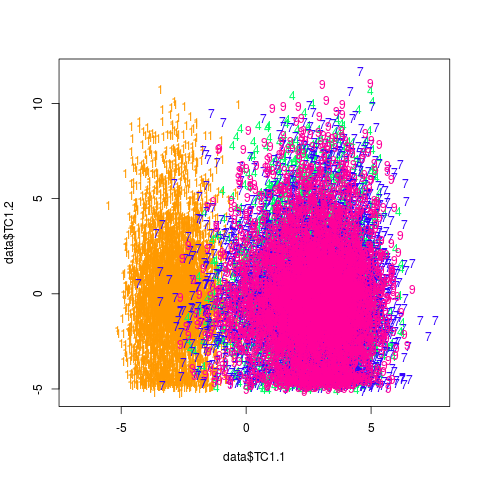
\includegraphics[scale=0.8]{exp5/PLS-2-1vs4vs7vs9}
	\caption{1 VS 4 VS 7 VS 9. Puntos en el nuevo espacio PLS-DA}
  \end{center}
\end{figure}

Finalmente analizaremos el tercer autod\'igito, en este caso son distintos para los dos m\'etodos. El de PCA se parece a un 3, mientras que PLS-DA se parece a un 6.

En este caso no mostraremos las matrices de confusi\'on, pero destacaremos que se siguen manteniendo las dos caracter\'isticas previas. Adem\'as notamos que la cantidad de aciertos sobre el total de casos de test es notablemente mayor para PLS-DA (66\% contra 50\%). Esto viene asociado con lo analizado en la secci\'on \ref{alpha-gamma}, pues PCA hasta el momento captur\'o el 23\% de la informaci\'on mientras que PLS-DA el 65\%.

Ahora mostraremos la distribuci\'on en este espacio de los puntos. Para mayores referencias:

\begin{figure}[h!]
  \begin{center}
	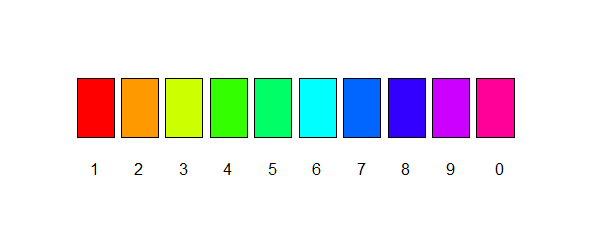
\includegraphics[scale=0.6]{exp5/AllVsAll/Referencias}
	\caption{Referencias de colores}
  \end{center}
\end{figure}

Los siguientes 8 gr\'aficos, corresponden, los primeros 4, a la distribuci\'on de los puntos seg\'un PCA y los \'ultimos 4, a la distribuci\'on seg\'un PLS-DA.

\begin{table}[h!]
\begin{subtable}{.5\linewidth}
\begin{tabular}{c}
	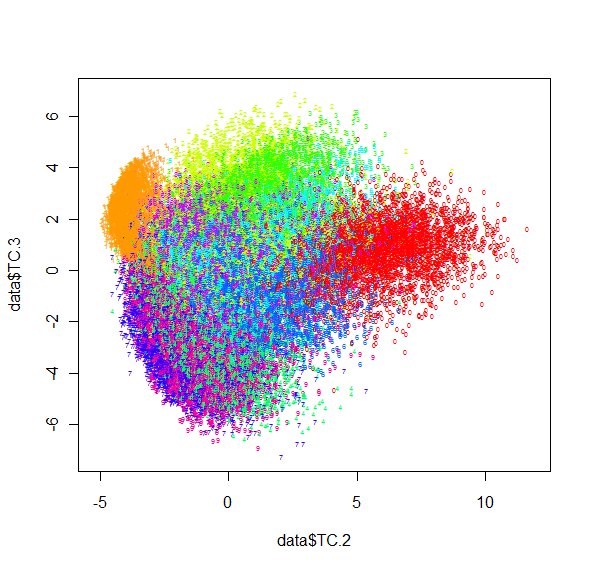
\includegraphics[scale=0.4]{exp5/AllVsAll/PCA-23}
\end{tabular}
\end{subtable}
\begin{subtable}{.5\linewidth}
\begin{tabular}{c}
	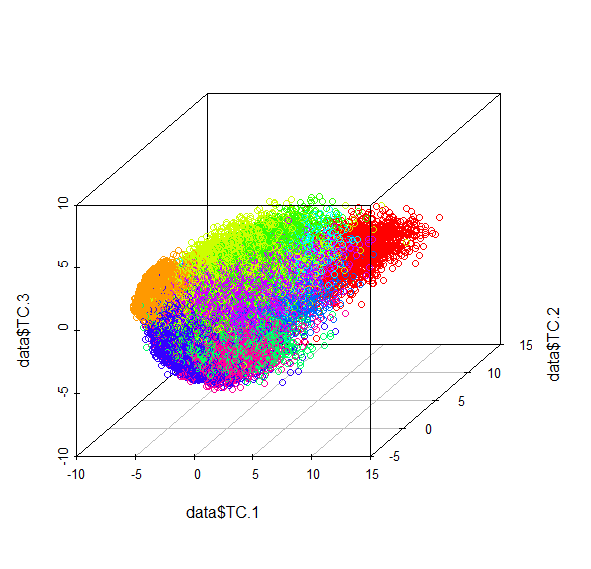
\includegraphics[scale=0.4]{exp5/AllVsAll/PCA-123}
\end{tabular}
\end{subtable}
\end{table}
\begin{table}[h!]
\begin{subtable}{.5\linewidth}
\begin{tabular}{c}
	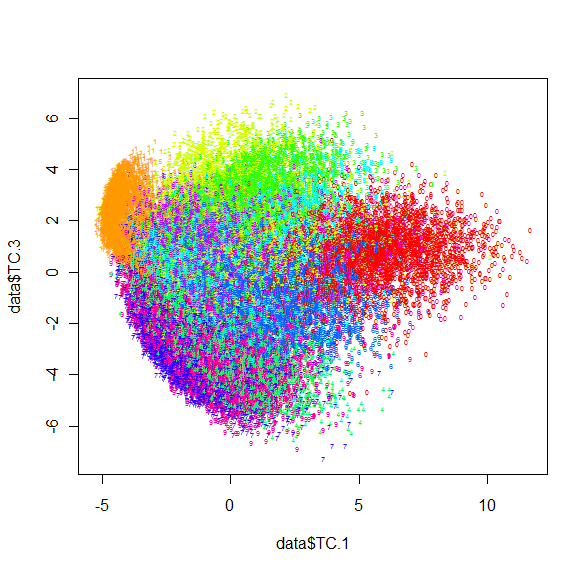
\includegraphics[scale=0.4]{exp5/AllVsAll/PCA-13}
\end{tabular}
\end{subtable}
\begin{subtable}{.5\linewidth}
\begin{tabular}{c}
	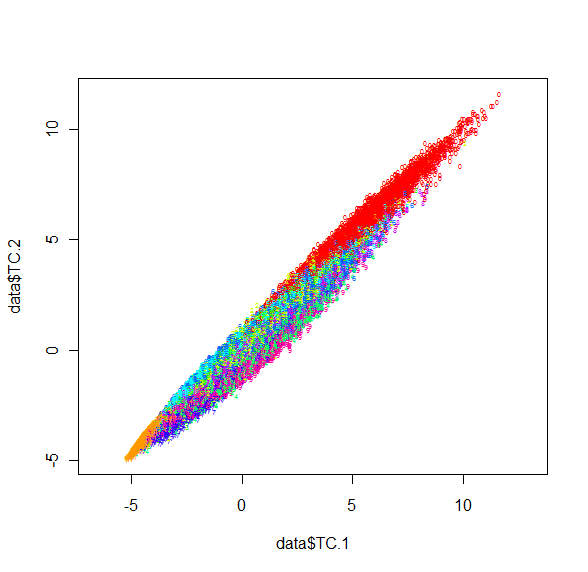
\includegraphics[scale=0.4]{exp5/AllVsAll/PCA-12}
\end{tabular}
\end{subtable}
\end{table}

\newpage

\begin{table}[h!]
\begin{subtable}{.5\linewidth}
\begin{tabular}{c}
	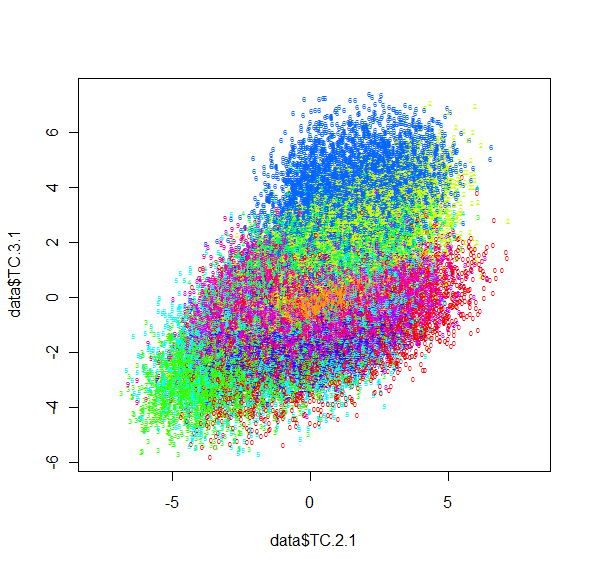
\includegraphics[scale=0.4]{exp5/AllVsAll/PLS-23}
\end{tabular}
\end{subtable}
\begin{subtable}{.5\linewidth}
\begin{tabular}{c}
	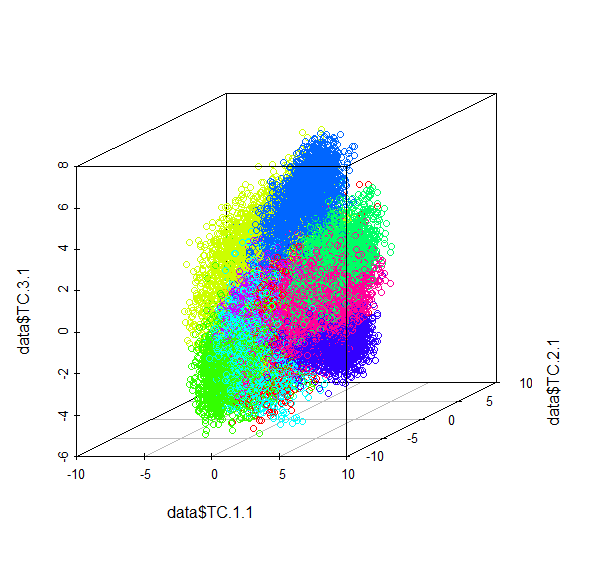
\includegraphics[scale=0.4]{exp5/AllVsAll/PLS-123}
\end{tabular}
\end{subtable}
\end{table}
\begin{table}[h!]
\begin{subtable}{.5\linewidth}
\begin{tabular}{c}
	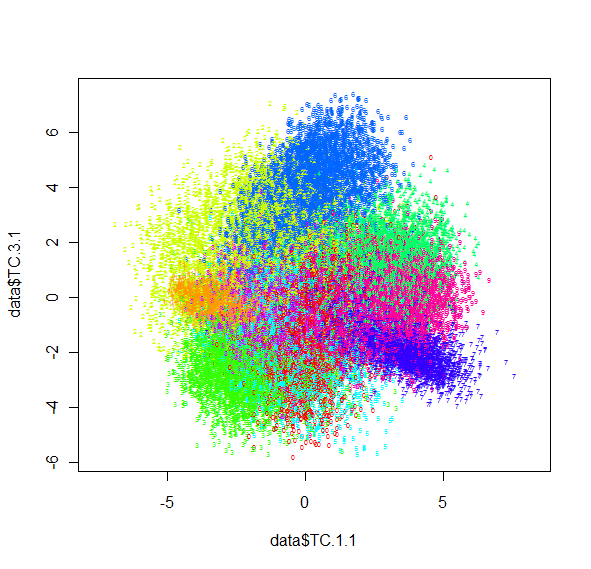
\includegraphics[scale=0.4]{exp5/AllVsAll/PLS-13}
\end{tabular}
\end{subtable}
\begin{subtable}{.5\linewidth}
\begin{tabular}{c}
	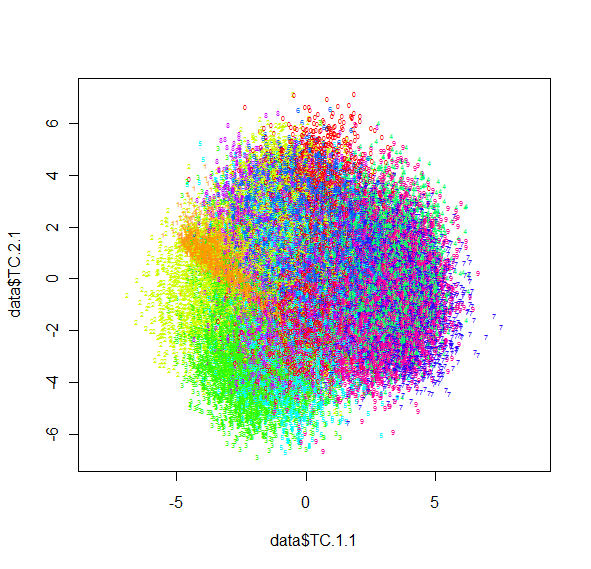
\includegraphics[scale=0.4]{exp5/AllVsAll/PLS-12}
\end{tabular}
\end{subtable}
\end{table}

En ambos se ve como se empiezan a formar burbujas donde se concentran los distintos d\'igitos. Como se dijo anteriormente, en PLS-DA es m\'as notorio. Los gr\'aficos que no son de las 3 dimensiones, corresponden a las proyecciones sobre alguno de los ejes, donde se ven algunas burbujas solapadas, pero que el gr\'afico 3D nos muestra que comienzan a separarse en los distintos planos.

Si bien no esperamos que las burbujas se separen por completo (tener un 100\% efectividad), s\'i esperamos que a mayor cantidad de dimensiones consideradas, alcancemos un hit-rate lo suficientemente alto en contraste al tiempo de ejecuci\'on de los algoritmos.